\section{Tipi di controlli sulle frodi}


\paragraph*{Controlli correttivi} (\textit{Corrective Controls})\\
Risolvono i problemi e prevengono problemi futuri.

\paragraph*{Controlli Rivelativi} (\textit{Detecive Controls})\\
Segnalano un warning quando un altro controllo di sicurezza viene bucato.

\paragraph*{Controlli preventivi} (\textit{Preventive Controls})\\
Prevengono le frodi. Includono: \textit{risk assessment}, sviluppo di controlli
interni, sicurezza fisica e informatica, autorizzazioni (es. password) e
\textit{segregation of duties}.

I controlli eseguiti in maniera preventiva sono migliori rispetto alle
altre tipologie di controlli.

La sicurezza fisica, come la protezione di alcuni locali all'interno
dell'azienda (es. sala server) va sempre tenuta in
considerazione e non va trascurata.

\subsection{Tecniche per scoraggiare una frode}

L'aspetto motivazionale è molto spesso da tenere in considerazione.
Un utente che esce con un alto grado di studio potrebbe subire delle
frustrazioni se gli viene assegnato un lavoro troppo basso per il suo livello.

Altro errore da non sottovalutare è la promozione: dopo 8 anni di solito una
persona si aspetta di essere promossa.

L'esempio è anche importante: le persone nell'alta gerarchia diventano un
\textbf{role model}, ovvero i sottoposti prendono ispirazione dai dirigenti, ed
è quindi fondamentale che essi abbiano un comportamento esemplare.

Ma come si rimuove la possibilità di una frode?
\begin{itemize}
  \item \textit{Segregation of duties};
  \item Sicurezza dei beni;
  \item Sicurezza fisica (es. sono presenti tornelli per accedere a determinate
aree per esempio?) (ISO 27000, CISA, CISP);
  \item \textit{Background checks}, spesso eseguiti su: titoli di studio,
  casi penali o precedenti esperienze lavorative.
\end{itemize}

\subsubsection{Segregation of Duties}

Bisogna fare in modo che il potere associato ad una certa funzione non risieda
nelle mani di una sola persona:
Esistono tre fondamenti per una corretta \textbf{segregation of duties}:
\begin{itemize}
  \item Origine;
  \item Autorizzazione;
  \item Verifica.
\end{itemize}

Se questi tre punti sono eseguiti correttamente (da tre persone diverse),
è molto difficile che una frode avvenga.
In caso avvenga, c'è di sicuro un caso di collusione.

\begin{figure}[H]
 \centering
 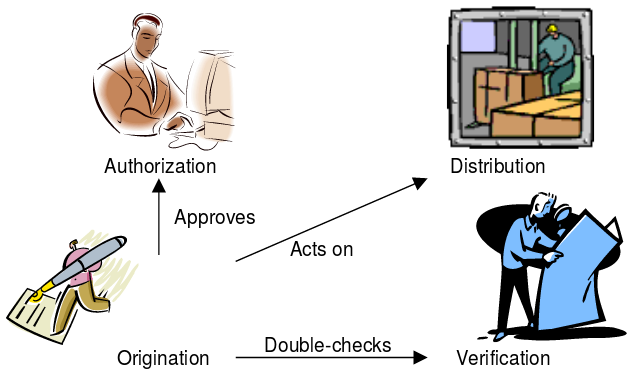
\includegraphics[scale=0.425]{segregation}
 \caption{Una corretta applicazione della \textbf{segregation of duties} con
quattro componenti.}
\end{figure}


\paragraph*{Controlli compensativi}

Questi tipi di controlli compensano l'assenza di alcuni controlli che possono
essere mancanti o difettosi, o quando la \textit{segregation of duties} non è
possibile. Queste tipologie di controlli sono spesso trasversali.

\subsection{Software per trovare frodi}

Fin dall'inizio del commercio, si iniziò a fare i controlli sui conti. Il
primo tipo di controllo implementato prima dell'arrivo dei computer era la
partita doppia. Ora con il computer sono presenti diversi tipi di software
per trovare delle frodi. Quelli di tipo finanziario vanno per la maggiore.



Per rilevare delle frodi un software può fare dei controlli
per evidenziare diversi segnali d'allarme come per esempio:
\begin{itemize}
\item confrontare gli indirizzi e i numeri di telefono dei venditori con
quelli dei dipendenti;
\item identificare i vari \textit{outlier}, ovvero tutto ciò che si
comporta molto diversamente rispetto alla media.
\end{itemize}
Il vantaggio dei controlli software è che vengono analizzati moltissimi
dati in brevi lassi di tempo. Nonostante questo, alcuni dati vengono
analizzati meglio da persone familiari con le operazioni dell'azienda,
con i venditori e con i sistemi di contabilità.
Queste persone possono ricercare venditori sconosciuti, beni o servizi
inusuali e acquisti eccessivi di servizi.

\subsection{Business Application Checks}
Gli assegni dovrebbero essere tenuti in un luogo con accesso ristretto e
se ne dovrebbe fare l'inventario almeno ogni trimestre.
Le informazioni di nuovi venditori dovrebbero essere ricontrollate
dal \textit{management}. In caso ci siano assegni restituiti,
questi devono essere mandati ad un PO Box e valutati da qualcuno esterno
all'azienda.

\paragraph*{PO Box}

È quello che si definisce un fermo posta, viene dato dall'ufficio postale
presentandosi con un documento d'identità. Il fermo posta non è associato a un
indirizzo di un'abitazione.

\subsection{Incoraggiare la sicurezza nei dipartimenti IT}

Alcuni punti focali:
\begin{itemize}
  \item Sicurezza fisica;
  \item \textit{Segregation of duties}: una cosa importante da non sbagliare è
  di mettere i controlli di monitoring
  sullo stesso hardware in cui si ha il software in produzione;
  \item Monitor dei dipendenti;
  \item Audit a sorpresa;
  \item Rotazione dei lavori;
  \item Analisi della documentazione.
\end{itemize}

\subsection{Esercizi}

Gli esercizi su questa parte sono presenti nella rispettiva Sezione
\ref{EsFrodi2}.


\section{Social Engineering}

Oggi è più facile eseguire un'\textit{escalation} di privilegi dall'interno,
piuttosto che tentare di entrare nel sistema in maniera non autorizzata.

Esempi tipici di attacchi che sfruttano la tenica del
\textit{Social Engineering} sono:
\begin{itemize}
  \item Le e-mail con degli allegati eseguibili;
  \item Le prime 500 persone a registrarsi a questo sito web vinceranno dei
  biglietti;
  \item Il tuo account è stato bloccato, per favore riesegui il login;
  \item Fingersi un tecnico IT\footnote{Richiede tempo ma permette di
introdursi all'interno dell'azienda. Il veicolo di questo attacco è la
fiducia.}.
\end{itemize}

\paragraph*{Definizione} Il \textit{social engineering} è convincere le persone
a fare cose che solitamente non farebbero.

\subsection{Come combattere il Social Engineering}

È importante essere aderenti alle procedure di verifica, che possono essere:
\begin{itemize}
  \item Verificare sempre che l'indirizzo e-mail sia dell'azienda;
  \item Verificare che il richiedente sia un impiegato e che ricopra
  effettivamente quel ruolo;
  \item Verificare l'autorizzazione richiesta;
  \item Verificare i record delle transazioni.
\end{itemize}

Anche a livello organizzativo è necessario applicare delle verifiche, che
potrebbero essere:
\begin{itemize}
  \item Classificazione dei dati e definizione del loro trattamento;
  \item \textit{Policies} definite per il comportamento degli impiegati;
  \item Addestramento dei dipendenti riguardo ai ruoli e alle \textit{policies}
che devono essere applicate.
\end{itemize}

\section[Statistiche sulle frodi]{
Statistiche sulle frodi\protect\footnote{
Le stime qui riportate sono state estratte dal libro
\textit{The Art of Steals} (2001). Si riferiscono
a quell'anno e pertanto non sono da considerare attuali.
Vengono riportate perché sono un utile strumento per
comprendere l'argomento.}}
Ogni anno negli Stati Uniti il business perde $400$ miliardi di dollari
per via delle frodi. Questa cifra corrisponde a due volte il budget
militare degli USA.
Un terzo di questo denaro è dovuto al fenomeno
dell'\textit{emblezzlement}, ovvero quando impiegati rubano ai propri
datori di lavoro.
Il problema è che molti dirigenti, per via dell'imbarazzo,
invece di riportare questi furti alla polizia, procedono con
il licenziamento, facendo sì che queste persone vadano a rubare da
qualcun altro.
Secondo il report di KPMG del 2000 altre cause importanti sono
la falsificazione di assegni, fatture false, clonazione di carte di
credito e i furti.

Un altro problema di fondamentale importanza è la \textbf{merce
contraffatta}.
Questo tipo di frode causa ogni anno una perdita
di $350$ miliardi di dollari negli USA.
La merce contraffatta che rende di più sono i medicinali.
Di solito le persone pensano che non sia un loro problema,
perché non si tratta di reati contro la persona, ma
invece colpisce tutti perché comporta un innalzamento delle tasse
per garantire beni e servizi.


Anche il furto d'identità costituisce una grossa frode, soprattutto negli
Stati Uniti, in cui basta il \emph{social security number} e un telefono per
aprire un conto a nome della vittima.

\section{Esercizi riassuntivi}

Gli esercizi riassuntivi su tutto il capitolo possono essere trovati nella
sezione apposita (\ref{EsFrodi3}).




\chapter{Business Continuity and Disaster Recovery}
\label{BCDR}

Prendiamo ad esempio una delle seguenti aziende:
\begin{itemize}
  \item 1 milione di account, carte di credito, prestiti;
  \item Società di Airline, con 250 voli giornalieri;
  \item Farmacia con 5 milioni di prescrizioni all'anno;
  \item Fabbrica con 200 impiegati che producono 200,000 prodotti.
\end{itemize}

Che cosa succede quando avviene un fallimento di sistema, come una interruzione
di corrente prolungata o un fallimento di server?

\section{Primo passo: Business Impact Analysis (BIA)}

È di fondamentale importanza analizzare l'impatto che un evento può avere sulla
società. Per capire questo, bisogna porsi la seguente domanda: qual è il
processo più critico dell'azienda?

Non è semplice rispondere a questa domanda, ma è necessario riuscire a
individuarlo.

È anche importante essere in grado di eseguire un'\textbf{analisi dei rischi},
da quelli più piccoli a quelli più grandi\footnote{Un meteorite, ad esempio}. È
anche doveroso chiedersi, come potrebbero questi eventi impattare sull'azienda?
Come si relazionano la safety e la security con questi rischi? E, infine,
quanto tempo impiego per recuperare ciò che ho perso? È possibile ritornare a
lavoro con due modalità: in modalità degradata o ritorno a lavorare a pieno
regime.

È da tenere conto che più velocemente si vuole tornare ad un regime di lavoro
normale più il costo aumenta.
